\documentclass[a3paper, 12pt]{article}

\usepackage[hscale=.9, vscale=.9]{geometry}
\usepackage{enumitem}
\usepackage{fix-cm}
\usepackage[none]{hyphenat}
\usepackage{graphicx}
\newcommand*\nfont{\fontsize{16}{19}\selectfont}

\parindent 0pt

%\hyphenation{distri-buted believe original other-wise}

\pagestyle{empty}

\begin{document}

% \vspace*{-5ex}
\begin{center}
  {\Huge 21st International Conference on}

  \medskip

  {\Huge Relational and Algebraic Methods in Computer Science}

  \bigskip

  {\fontsize{36}{50}\selectfont RAMICS 2024}

  \bigskip

  {\Huge Charles University, Prague, 19-23 August 2024}

  \medskip

  {\Huge Collocated with AiML}
  
  \bigskip

  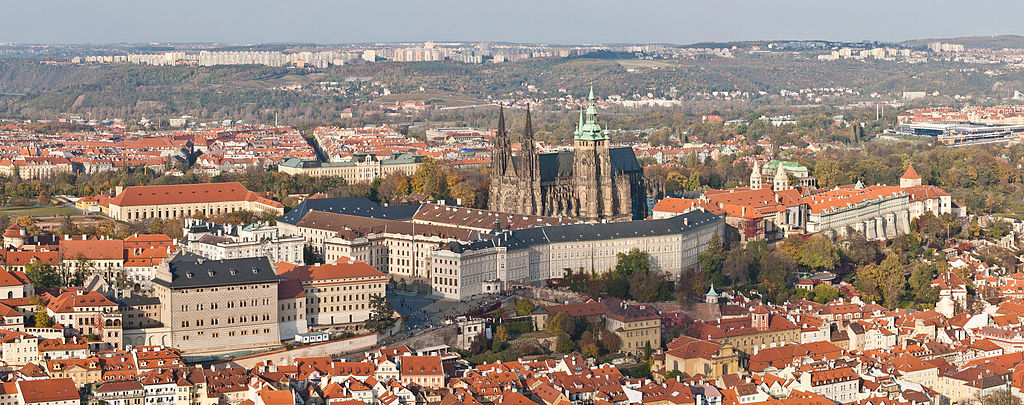
\includegraphics[width=.7\linewidth, trim=0 20 0 0, clip]{prague}

  \medskip
\end{center}

\begin{minipage}[t]{.473\linewidth}
  \nfont%
  Since 1994, the RAMICS conference series has been the main venue for
  research on relation algebras, Kleene algebras and similar algebraic
  formalisms, and their applications as conceptual and methodological
  tools in computer science and beyond.

  \medskip

  Theoretical aspects include semigroups, residuated lattices,
  semirings, Kleene algebras, relation algebras, quantales and other
  algebras; their connections with program logics and other logics;
  their use in the theories of automata, concurrency, formal
  languages, games, networks and programming languages; the
  development of algebraic, algorithmic, category-theoretic,
  coalgebraic and proof-theoretic methods for these theories; their
  formalisation with theorem provers.

  \medskip

  Applications include tools and techniques for program correctness,
  specification and verification; quantitative and qualitative models
  and semantics of computing systems and processes; algorithm design,
  automated reasoning, network protocol analysis, social choice,
  optimisation and control.

  \bigskip

  {\Large \bf Call for Papers}

  \smallskip

  We invite original submissions in the general field of algebraic
  structures relevant to computer science and on applications of such
  algebras.  Submissions must be unpublished, not under review for
  publication elsewhere and provide sufficient information to judge
  their merits.

  The proceedings of RAMICS 2024 will be published in an LNCS volume
  by Springer.  As for earlier RAMICS conferences, we intend to
  publish a journal special issue with revised and extended versions
  of a selection of the best papers.
  
  \bigskip
  
  {\Large \bf Important Dates}

  \smallskip

  Abstract Submission (extended): \textbf{16 March 2024}
  
  Paper Submission (extended): \textbf{23 March 2024}
  
  Author Notification: 21 May 2024

  %Final Version: 1 June 2024
\end{minipage}
\hfill
\begin{minipage}[t]{.43\linewidth}
  \nfont%
  \hfill {\Large \bf Invited Speakers}

  \medskip

  \begin{minipage}{.2\linewidth}
    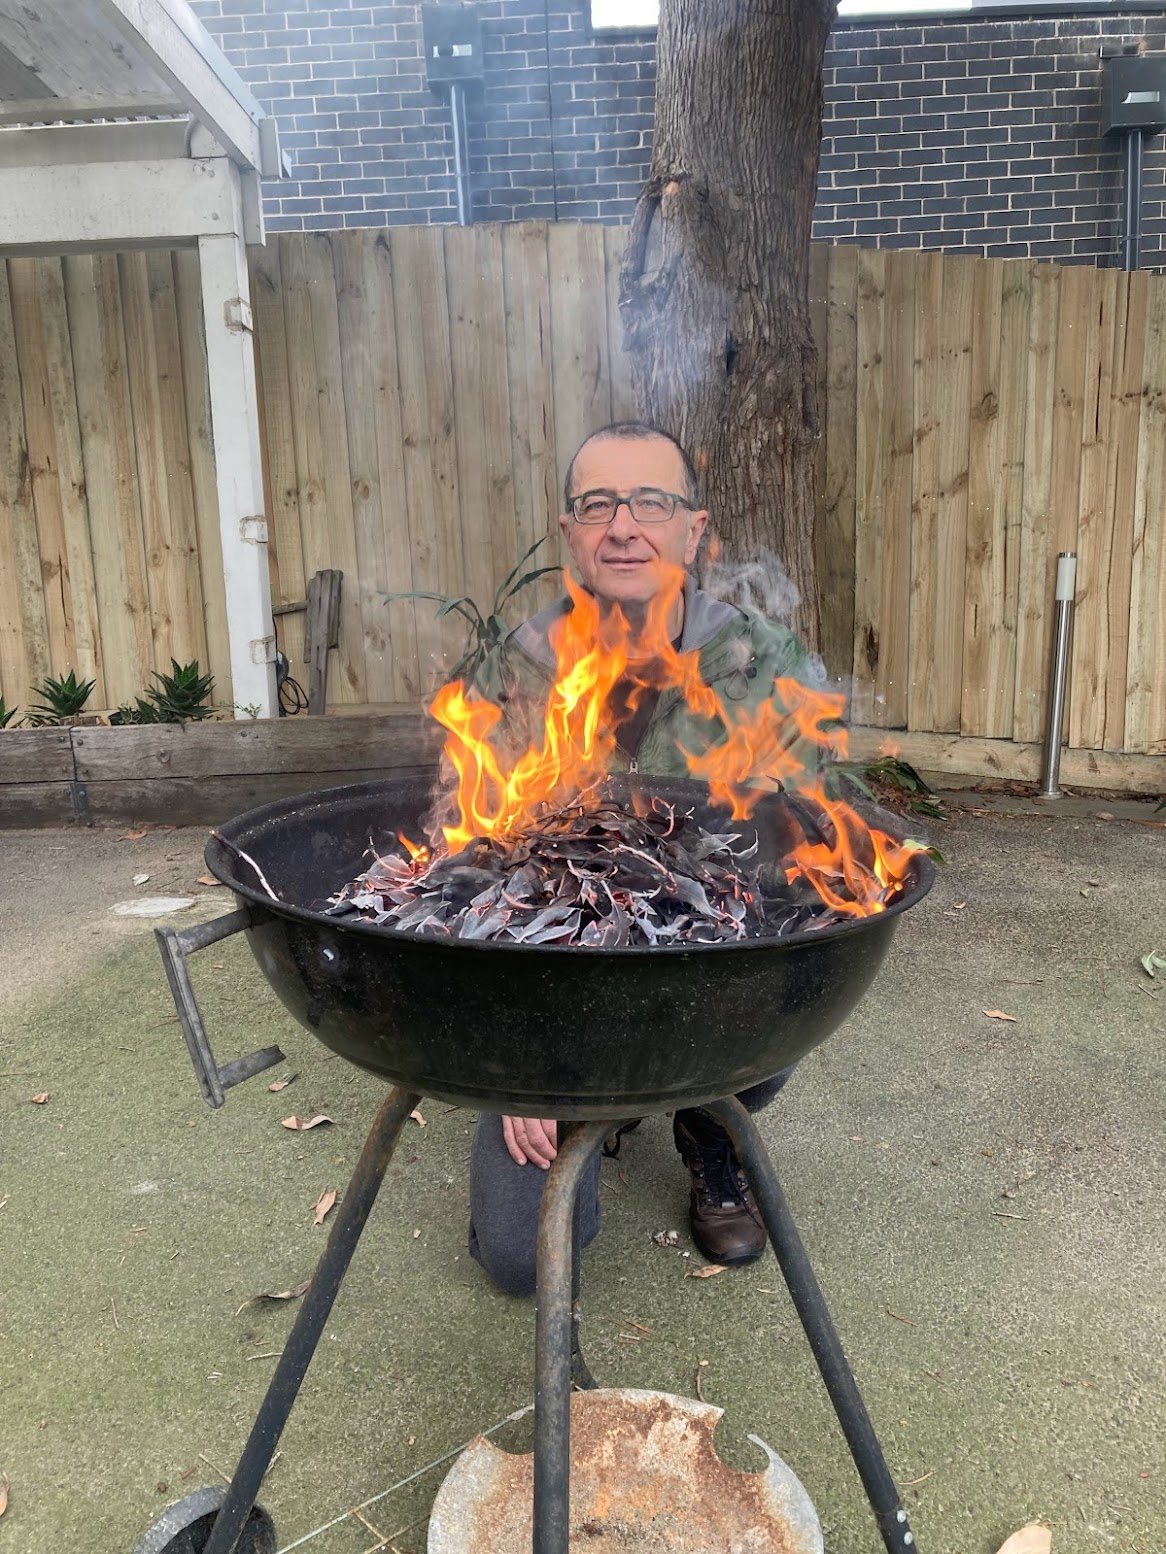
\includegraphics[width=\linewidth, trim=0 30 0 0, clip]{kowalski2}
  \end{minipage}
  \hfill
  \begin{minipage}{.75\linewidth}
    \textbf{Tomasz Kowalski}

    Jagiellonian University in Kraków

    Poland
  \end{minipage}

  \medskip

  % \begin{minipage}{1.0\linewidth}
  %   \flushleft%
  %   \textbf{Compositional synthesis of interconnected control systems}
  % \end{minipage}
  
  %\vspace{-2ex}
  \begin{minipage}{.75\linewidth}
    \flushright%
    \textbf{Sarah Winter}

    IRIF, Université Paris Cité

    France
  \end{minipage}
  \hfill
  \begin{minipage}{.2\linewidth}
    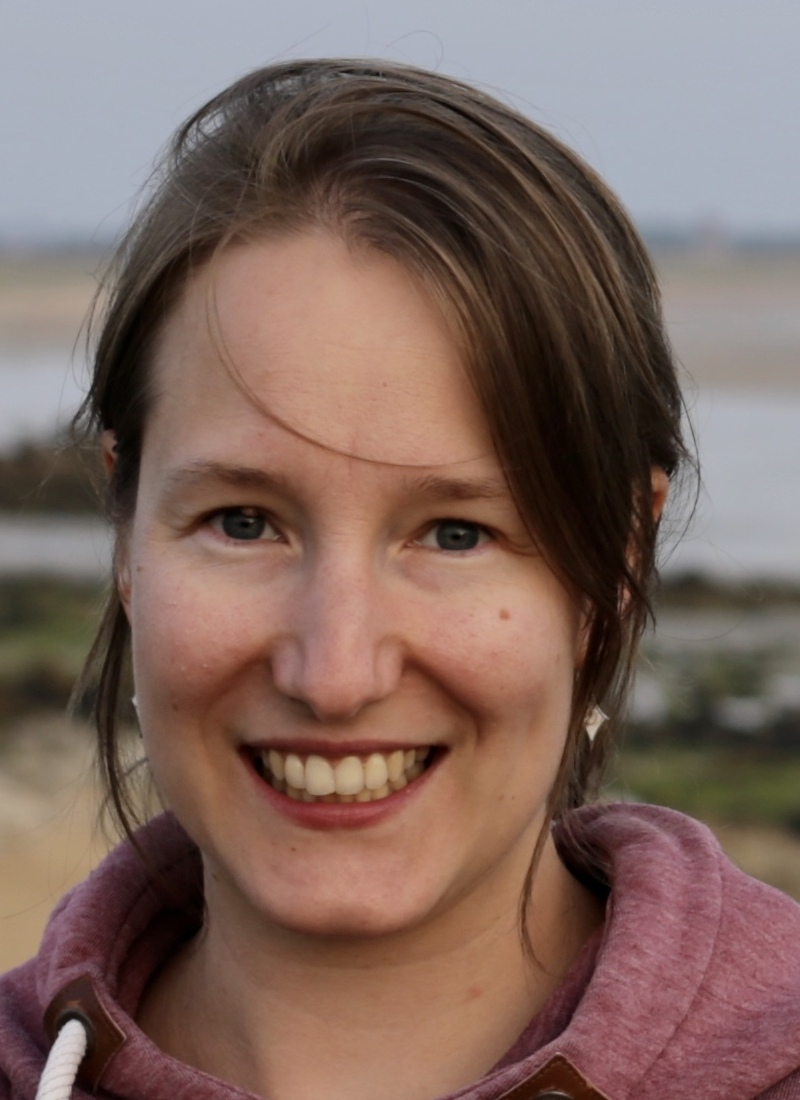
\includegraphics[width=\linewidth, trim=0 0 0 0, clip]{winter}
  \end{minipage}

  \medskip

  % \begin{minipage}{1.0\linewidth}
  %   \flushright%
  %   \textbf{Underwater robotics: past, present, and future}
  % \end{minipage}
  
  %\vspace{-2ex}
  \begin{minipage}{.2\linewidth}
    
\includegraphics[width=\linewidth, trim=15pt 0 0 0, clip]{goncharov2}
  \end{minipage}
  \hfill
  \begin{minipage}{.75\linewidth}
    \textbf{Sergey Goncharov}

    % Friedrich-Alexander
    University of Erlangen \& Nürnberg

    Germany
  \end{minipage}

  \medskip
  
  % \begin{minipage}{1.0\linewidth}
  %   \flushleft%
  %   \textbf{Swarms of mobile robots, towards safety with versatility}
  % \end{minipage}

  \vspace*{7ex}
  
  \hfill {\Large \bf Organization}

  \smallskip

  \hfill \textbf{Uli Fahrenberg}, EPITA, France

  \hfill \textbf{Wesley Fussner}, Czech Academy of Sciences,

  \hfill Prague, Czechia

  \hfill \textbf{Roland Glück}, German Aerospace Center,

  \hfill Augsburg, Germany

  \bigskip

  \hfill {\Large \bf Program Committee}

  \smallskip

  % \hspace*{-1em}
  % \begin{minipage}{1.1\linewidth}
  Roland Backhouse,
  Manuel Bodirsky,
  Xavier Caicedo Ferrer,
  Willem Conradie,
  Jules Desharnais,
  Jérémy Dubut,
  Marie Fortin,
  Hitoshi Furusawa,
  Valentin Goranko,
  Walter Guttmann,
  Robin Hirsch,
  Peter Höfner,
  Sebastiaan Joosten,
  Wolfram Kahl,
  Tobias Kappé,
  Roger Maddux,
  Dale Miller,
  Luigi Santocanale,
  Ana Sokolova,
  Jiři Srba,
  Sara Ugolini,
  Jana Wagemaker,
  Michael Winter,
  Krzysztof~~Ziemiański
  % \end{minipage}

  \vspace{8ex}

  \hspace*{-15ex} {\fontsize{30}{40}\selectfont https://ramics-conf.github.io/2024/}

  \vspace*{-2ex}

\end{minipage}

\end{document}
